\section{Introduction}
L'utilisation des systèmes de reconnaissance de la parole permet d'accéder à l'information de manière rapide et intuitive. Aujourd'hui, beaucoup de nos appareils électroniques ont une exploitation plus naturelle car ils embarquent des fonctionnalités de reconnaissance de la parole. Cependant, nous remarquons que ces systèmes traitent rarement la langue arabe de manière efficace.

Dans ce chapitre nous présentons l'état de l'art pour les systèmes de reconnaissance de la parole et notamment pour la langue arabe. Mais avant cela, nous définissons les différentes techniques et approches utilisées pour la conception des systèmes End-To-End et des systèmes basés reconnaissance de phonèmes pour la reconnaissance de la parole.

\section{Techniques utilisées pour l'approche End-To-End}
\cite{ml} définit l'apprentissage automatique comme étant un programme informatique qui apprend d'une expérience \textit{E} à l'égard de certaines classes de tâches \textit{T} et de la mesure de performance \textit{P}. Si sa performance aux tâches en \textit{T}, la performance mesurée par \textit{P}, s'améliore avec l'expérience \textit{E}.\\ En d'autres termes, l'apprentissage automatique est une technique d'intelligence artificielle basée sur différentes notions mathématiques et plus particulièrement statistiques. Elle permet aux ordinateurs d'apprendre à partir des données et résoudre des problèmes ou effectuer des tâches complexes sans être explicitement programmés à cet effet \cite{Goodfellow-et-al-2016}.

L'apprentissage automatique se présente sous plusieurs types et ce en fonction du problème et du jeu de données à disposition. Ces types sont l'apprentissage supervisé, l'apprentissage non supervisé et l'apprentissage par renforcement \cite{typesml}. Pour la conception de notre système, nous nous intéressons au paradigme d'apprentissage supervisé.

L'apprentissage est dit supervisé lorsque le système apprend à classer des données à partir d'un algorithme d'entraînement\footnote{Nous utilisons pour la suite de ce document l'expression : Algorithme d'apprentissage}, traduit de "training" en anglais, ainsi que des exemples de données connus \cite{supervised}. Ce type d'apprentissage se divise en deux parties :
\begin{itemize}
    \item la première correspond à générer un modèle ayant la capacité de prédire la classe d'un ensemble de données qu'il rencontre pour la première fois. La génération de ce modèle se fait grâce à un algorithme d'apprentissage ainsi qu'à des données étiquetées (labelisées), et
    \item la deuxième consiste à prédire l'étiquette d'une nouvelle donnée dont nous ignorons le label à partir du modèle préalablement généré. \\
\end{itemize}

Comme mentionné dans le chapitre précédent, l'architecture End-To-End se base sur différents types de réseaux de neurones pour permettre de prédire la transcription associée à une entrée audio. Ce choix d'algorithme d'apprentissage, en plus des avantages classiques des réseaux de neurones, se justifie par :\\
\begin{itemize}
    \item la capacité d'apprendre et de modéliser des relations complexes et non-linéaires ce qui est le cas lorsqu'il s'agit d'associer du texte à de la parole, et
    \item contrairement à beaucoup d'autres techniques, certains réseaux de neurones tels que les réseaux récurrents n'imposent pas de restriction en terme de taille des données aux variables d'entrée. Dans notre cas, les données sont des séries chronologiques, traduit de Time Series en anglais, et se présentent sous forme de séquences de taille variable. Étant donné leur capacité à apprendre des relations cachées entre les données, les réseaux de neurones sont la solution de prédilection à notre problématique. \\
\end{itemize}

Nous présentons dans ce qui suit les différents types de réseaux de neurones ainsi que ce qu'ils peuvent apporter à notre tâche.

\subsection{Réseaux de neurones artificiels}
Les réseaux de neurones artificiels, ou Artificial Neural Networks (ANN) en anglais, sont des réseaux fortement connectés de processeurs élémentaires fonctionnant en parallèle. Chaque processeur élémentaire calcule une sortie unique sur la base des informations qu'il reçoit \cite{neuralnetsbook}. Ces réseaux artificiels sont inspirés de l'interconnexion des neurones chez les êtres vivants et sont composés d'une succession de couches où chacune prend ses entrées depuis les sorties de la couche précédente. 
De base, tout réseau de neurones est composé d'une couche d'entrée, une ou plusieurs couches cachées et une couche de sortie comme le montre la figure suivante \cite{neuralnetsbook} : 

\begin{figure}[H]
    \centering
    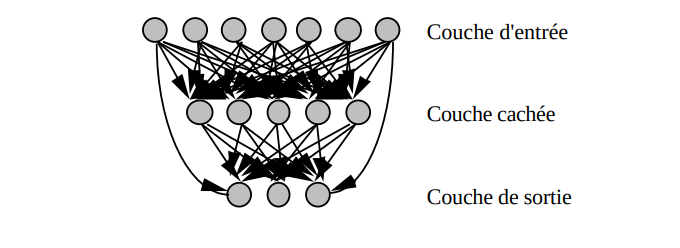
\includegraphics[height=150pt,width=325pt]{images/chap2/neural_net.png}
    \caption{Couches d'un réseau de neurones}
\end{figure}

Il existe plusieurs catégories de réseaux de neurones artificiels, \cite{neuralnetsbook} les classifie en : \\
\begin{itemize}
    \item \textbf{Réseaux multicouche} : Les connexions se font entre les neurones des couches en aval, et chaque neurone d'une couche est connecté à tous les neurones de la couche suivante et celle-ci seulement.
    \item\textbf{Réseaux à connexions locales} : Chaque neurone entretient des relations avec un nombre réduit et localisé de neurones de la couche avale.
    \item \textbf{Réseaux à connexion complète} : Structure d'interconnexion la plus générale où chaque neurone est connecté à tous les neurones du réseau.
\end{itemize}

\subsection{Réseaux de neurones profonds}
Les réseaux de neurones profonds, traduits de l'anglais Deep Neural Networks (DNN), sont des réseaux qui se composent de plusieurs couches cachées où chaque type de couche présente des avantages pour des cas d'utilisation spécifiques. Cependant, quelque soit l'architecture interne de ces réseaux, ces derniers partagent la même intuition des réseaux de neurones qui consiste à introduire des données et entraîner le modèle à interpréter ces dernières et à prédire un label qui, dans notre cas, est la transcription d'une entrée audio.

Dans le cas de l'architecture End-To-End du système de reconnaissance de la parole, nous nous intéressons aux réseaux de neurones récurrents et réseaux à convolutions.

\subsubsection{Réseaux de neurones récurrents}
Les réseaux de neurones récurrents, ou Recurrent Neural Networds (RNN) en anglais, font partie d'un groupe plus large d'algorithmes appelés modèles de séquence. Les modèles de séquence ont fait des pas de géant dans les domaines qui traitent des données séquentielles comme la reconnaissance de la parole, la génération de musique, l'analyse des séquences ADN ou encore la traduction automatique \cite{rnntowardsdata}. Les réseaux de neurones récurrents sont idéals pour appréhender ce genre de problèmes car contrairement aux réseaux de neurones classiques (ou encore les réseaux à convolutions que nous présentons dans ce qui suit), ces réseaux sont conçus pour prendre une série d'entrées sans déterminer leur taille au préalable. \\
Le point fort des RNNs reste néanmoins leur capacité à mémoriser les suites de séquences de données ce qui s'avère essentiel pour la reconnaissance de la parole \cite{rnnintro}. En effet ces réseaux se souviennent des séquences de données passées et la décision à prendre (classification par exemple) est influencée par ce qui a été appris du passé et ce grâce à une composante de ce réseau qui est le vecteur d'états cachés ou Hidden States Vector en anglais. 

La figure suivante \cite{rnnschema} détaille le flux de l'information dans ce réseau.
\begin{figure}[H]
    \centering
    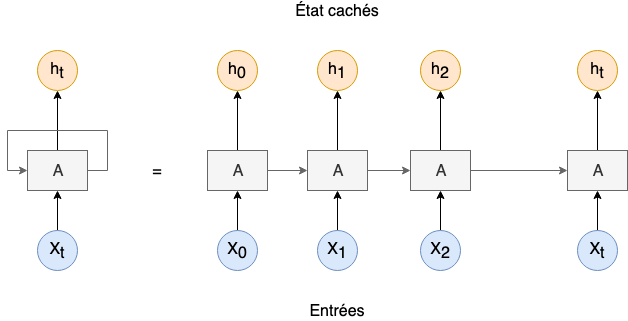
\includegraphics[height=175pt,width=300pt]{images/chap2/RNN.png}
    \caption{Réseau de neurones récurrent}
\end{figure}

Nous remarquons donc qu'à chaque timestep \footnote{Timestep : Pas de temps ou découpe temporelle d'une donnée}, le RNN génère un output ainsi qu'un vecteur d'états cachés qui fera office d'input pour le prochain timestep. \\
Le vecteur d'états cachés est une représentation abstraire du séquencement des données et c'est cette information qui permet au réseau de prendre en compte les informations précédentes à l'instant \textbf{t}. Il est cependant important de noter que les RNNs souffrent, lorsque la taille des séquences est suffisamment grande, du problème du \textit{Vanishing Gradient} qui arrive lorsque les poids du modèle ne sont plus mis à jour et que le gradient avoisine le zero. Il existe néanmoins d'autres réseaux tel que les LSTMs\footnote{Long Short-Term Memory : type de réseau récurrent que nous détaillons dans le chapitre suivant.} basés sur le principe des réseaux de neurones récurrents et qui évitent le \textit{Vanishing Gradient} \cite{vanishinggradient}.  

\subsubsection{Réseaux de neurones à convolutions}
Les réseaux de neurones à convolutions, ou Convolutional Neural Networks (CNN) en anglais, ont été introduits par \cite{cnnhist} et sont analogues aux réseaux de neurones classiques car ils sont composés de neurones qui s'auto-optimisent par l'apprentissage \cite{cnnintro}. L'une des plus grandes limitations des réseaux de neurones traditionnels est qu'ils ne donnent pas de bon résultats avec des données multi-dimensionnelles au vu de  la complexité de calcul et c'est là où réside la grande différence entres les réseaux à convolutions et les ANNs. Un CNN est capable de capturer avec succès les dépendances spatiales et temporelles des données grâce à l'application de filtres appropriés. L'architecture s'ajuste mieux aux données spatiales ou encore séquentielles en raison de la réduction du nombre de paramètres impliqués comme c'est le cas des images, des vidéos ou encore du son comme dans notre cas. Dans un CNN, deux opérations sont appliquées : 
\begin{itemize}
    \item \textbf{Convolution :} Consiste à appliquer un masque de convolution de taille \textbf{(M $\times$ M)} sur l'image en spécifiant un nombre de filtres afin d'extraire les informations pertinentes sous forme d'un ensemble de matrices (ou de filtres) de taille \textbf{(N-M+1 $\times$ N-M+1)}.    
    \item \textbf{Pooling :} Il existe deux variantes pour cette opération: Pooling Maximum et Pooling Moyen. Cette opération consiste à appliquer un masque de taille \textbf{(M $\times$ M)} à la matrice et ne garder que le maximum ou la moyenne de ce masque selon que nous appliquons un Pooling Maximum ou moyen et générer un ensemble de matrices de taille \textbf{(N/M $\times$ N/M)}.\\
\end{itemize}

La figure suivante illustre le fonctionnement d'un réseaux de neurones à convolution à travers un exemple numérique pour une image en 2D.
\begin{figure}[H]
    \centering
    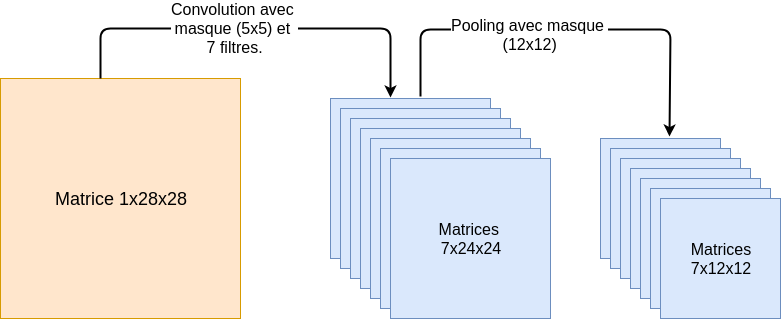
\includegraphics[height=150pt,width=300pt]{images/chap2/CNN.png}
    \caption{Réseau de neurones à convolution}
\end{figure}

Dans le cadre de ce projet, nous traitons des enregistrements audio qui sont des données de type séries temporelles, ces données sont sous forme de vecteurs d'attributs nous utilisons donc des réseaux de neurones à convolution en 1D \cite{cnn1d}. La logique de fonctionnement de ces réseaux est la même à la différence que les masques de convolution et de pooling sont des vecteurs en une dimension au lieu de matrices en deux dimensions pour le cas des images.

\section{Approches utilisées pour les systèmes de reconnaissance basés reconnaissance de phonèmes}
\subsection{Modèle acoustique}  
\subsubsection{Modèles de Markov Cachés}
Traduit de Hidden Markov Models (HMM), les Modèles de Markov Cachés est une approche probabiliste permettant de représenter des distributions de probabilités à partir d'une chaîne d'observations. Par définition, un modèle de Markov caché est un processus doublement stochastique avec un processus sous-jacent non observable (processus caché) mais pouvant uniquement être observé au moyen d'un autre ensemble de processus stochastiques produit à partir de la séquence d'événements observée \cite{hmmdef}. Ces modèles sont basés sur deux propriétés. Premièrement, l'observation à l'instant \textit{t} a été générée par un processus dont l'état \textit{S} est caché à l'observateur. Deuxièmement, nous supposons que l'état du processus caché satisfait la propriété de Markov qui dit qu'étant donné la valeur de l'état \textit{$S_{t-1}$}, l'état actuel \textit{$S_{t}$} est indépendant de tous les états antérieurs à \textit{t - 1}. En d'autres termes, à un moment donné, l'état résume tout ce que nous devons savoir sur l'historique du processus afin de prédire son avenir \cite{hmmdef2}.

Afin d'illustrer ce que nous venons d'expliquer nous prenons l'exemple suivant \cite{hmmexample} : 
\begin{figure}[H]
    \centering
    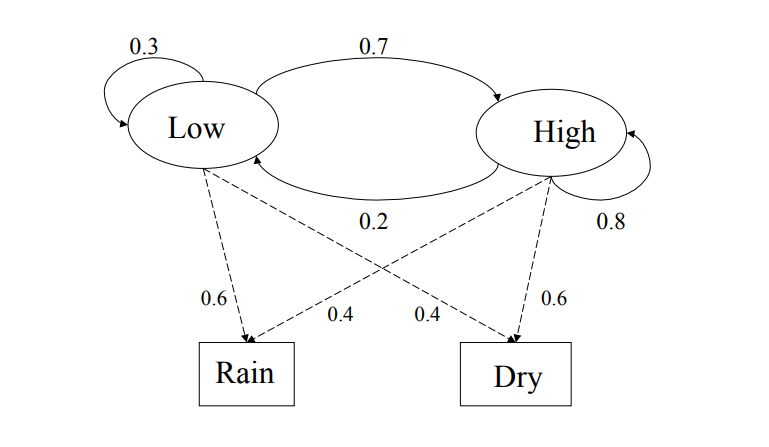
\includegraphics[width=350pt]{images/chap2/hmm_example.png}
    \caption{Exemple Modèle de Markov Caché}
\end{figure}

\begin{itemize}
    \item High et Low sont les états et Rain et Dry sont les observations.
    \item Les probabilités de transition sont : P(Low|Low)=0.3 , P(High|‘Low)=0.7 ...
    \item Les probabilités d'obvservation sont : P(‘Rain'|‘Low')=0.6, P('Dry'|'Low')=0.4 ...
    \item Les probabilités initiales sont : P('Low')=0.4, P('High')=0.6.
\end{itemize}

Une chaîne de Markov Caché nous permet de calculer la probabilité d'une séquence d'observations. Dans le cas de la reconnaissance de la parole nous utilisons cette propriété pour calculer la probabilité de d'avoir une suite de phonèmes sachant un ensemble d'observations (le spectrogramme) et un ensemble d'états (les phonèmes).
Afin de tirer profit des HMMs pour la conception du modèle acoustique, nous avons besoin du vecteur de distributions de probabilités. Pour cela nous pouvons utiliser des Modèles de Mélange Gaussien.

\subsubsection{Modèles de Mélange Gaussien}
Traduit de "Gaussian Mixture Models (GMM)", les Modèles de Mélange Gaussien consistent en une fonction de densité de probabilité paramétrique représentée par la somme pondérée de valeurs Gaussiennes.

Les GMMs sont couramment utilisés comme modèle paramétrique de la distribution de probabilité de mesures ou de caractéristiques continues dans un système biométrique, telles que les caractéristiques spectrales liées au tract vocal dans un système de reconnaissance de la parole \cite{gmmdef}.

Les GMMs permettent de calculer la vraisemblance de variables aléatoires continues offrent ainsi la possibilité de modéliser les distributions de probabilités sur des vecteurs d'entités en entrée associés à chaque état d'un HMM.
Malgré tous leurs avantages, les GMMs présentent un grave inconvénient: ils sont statistiquement inefficaces pour modéliser des données situées sur ou à proximité d'une variété non linéaire dans l'espace de données \cite{dlacoustic}. Dans le cas des systèmes de reconnaissance de la  parole, le discours est produit en modulant un nombre relativement réduit de paramètres, ce qui implique que sa véritable structure sous-jacente est beaucoup plus petite que ce qui apparaît immédiatement dans un vecteur contenant des centaines de caractéristiques.


\subsection{Modèle de langage}
Dans un système de reconnaissance de la parole, un modèle de langage peut être créée à partir du principe de N-gramme. Un N-gramme est une suite de \textit{N} caractères, mots ou même phonèmes qu'on peut retrouver dans une chaîne de caractères ou plus généralement dans un texte \cite{speechlangprocessing}. À titre d'exemple, la phrase : "ce projet est passionnant" contient :
\begin{itemize}
    \item Quatre 1-grammes (ou Uni-grammes) qui sont des chaînes de caractère de longueur de un mot à savoir : "ce", "projet", "est" et "passionnant".
    \item Trois 2-grammes (ou Bi-grammes) qui sont : "ce projet", "projet est" et "est passionnant".
    \item Deux 3-grammes (ou Tri-grammes) qui sont : "ce projet est" et "projet est passionnant".
    \item Un 4-grammes qui est la phrase entière.\\
\end{itemize}

Le choix du N-gramme à utiliser dépend de la structure de la langue que nous voulons traiter (la langue arabe dans notre cas). Utiliser un N-gramme avec un \textit{N} trop petit risquerait de ne pas permettre au modèle de langage de détecter les incohérence dans les suites de phonèmes reconnues par le modèle acoustique. Par ailleurs, si la suite de mots est trop longue nous pouvons nous retrouver dans un cas de sur-apprentissage\footnote{Désigne le fait qu'un modèle s'adapte bien aux données d'apprentissage et présente de très bons résultats mais, présente des résultats bien inférieurs une fois face à des données qu'il n'a jamais croisé \cite{underoverfitting}.} et donc de mémoriser les phonèmes associés à une entrée audio rencontrée pendant la phase d'entraînement mais donner de mauvais résultats pour de nouvelles entrées audio non rencontrées.

\section{Mesures de performances}

Il existe plusieurs mesures possibles pour évaluer la performance d'un système de reconnaissance de la parole.
Nous présentons les quatre métriques que nous utiliserons pour la suite de ce mémoire afin d'évaluer différents systèmes et architectures.

\subsection{Taux d'erreur des mots}
Le taux d'erreur de mots, traduit de Word Error Rate (WER) en anglais, est utilisé pour la reconnaissance continue des mots et où la taille d'une séquence n'est pas prédéfinie. Cette mesure est calculée à partir de la formule suivante \cite{werformula} : \\
        \begin{equation}
            WER = \frac{S + D + I}{N}
        \end{equation}
        où :\\
        S : nombre de mots qui ont été substitués lors de la reconnaissance.\\
        D : nombre de mots qui n'ont pas été écoutés ou ont plutôt été supprimés.\\
        I : nombre de mots qui ont été rajoutés sans qu'ils soient présents dans la parole.\\
        N : nombre total de mots de l'entrée.
        
\subsection{Taux d'erreur de caractères}
Le taux d'erreur de caractères, traduit de Character Error Rate CER en anglais, est une mesure similaire à la métrique WER. Celle ci est généralement utilisée pour mesurer la performance de l'architecture End-To-End où le résultat de la reconnaissance peut être une suite de caractères. Cette mesure est calculée à partir de la formule suivante : \\
        \begin{equation}
            CER = \frac{S + D + I}{N}
        \end{equation}
        où :\\
        S : nombre de caractères qui ont été substitués lors de la reconnaissance.\\
        D : nombre de caractères qui n'ont pas été écoutés ou ont plutôt été supprimés.\\
        I : nombre de mots qui ont été rajoutés sans qu'ils soient présents dans la parole.\\
        N : nombre total de caractères de l'entrée.

\subsection{Exactitude des mots}
L'exactitude des mots ou, Word Accuracy en anglais, est une mesure que nous utilisons lors de  l'entraînement de notre modèle afin de visualiser la performance de ce dernier et ainsi modifier les paramètres utilisés en fonction du besoin. Cette mesure est calculée à partir de la formule suivante :\\ 
    \begin{equation}
    WAcc = 1 - WER = \frac{N - S - D - I}{N} = \frac{H - I}{N}
    \end{equation}
    où : \\
        S : nombre de mots qui ont été substitués lors de la reconnaissance.\\
        D : nombre de mots qui n'ont pas été écoutés ou ont plutôt été supprimés.\\
        I : nombre de mots qui ont été rajoutés sans qu'ils soient présents dans la parole.\\
        N : nombre total de mots de l'entrée.\\    
        H : nombre de mots correctement reconnus.

\subsection{Exactitude des caractères}
L'exactitude des caractères ou, Character Accuracy en anglais, est une mesure que nous utilisons lors de  l'entraînement de notre modèle afin de visualiser la performance de ce dernier et ainsi modifier les paramètres utilisés en fonction du besoin. Cette mesure est calculée à partir de la formule suivante :\\ 
    \begin{equation}
    CAcc = 1 - CER = \frac{N - S - D - I}{N} = \frac{H - I}{N}
    \end{equation}
    où : \\
        S : nombre de caractères qui ont été substitués lors de la reconnaissance.\\
        D : nombre de caractères qui n'ont pas été écoutés ou ont plutôt été supprimés.\\
        I : nombre de caractères qui ont été rajoutés sans qu'ils soient présents dans la parole.\\
        N : nombre total de caractères de l'entrée.\\    
        H : nombre de caractères correctement reconnus.


% \subsection{Mesure pour les systèmes de questions-réponses}
% La métrique que nous utilisons pour évaluer la performance d'un système de questions-réponses est le Rang Réciproque Moyen.\\
% Traduit de "Mean Reciprocal Rank (MRR)", le Rang Réciproque Moyenf  est une mesure statistique permettant d'évaluer tout processus produisant une liste de réponses possibles à un échantillon de questions. Ces réponses sont classées par probabilité d'exactitude\cite{MRR}.\\
% Le MRR est calculé comme suit: \\ 
% \begin{center}
%   MRR = $\sum_{i=1}^{n}\frac{1}{R_{i}}$ 
% \end{center}
% où :
% \begin{itemize}
%     \item n : le nombre de questions du test
%     \item $R_{i}$ : le rang de la première réponse correcte pour la i\_eme question du test.
% \end{itemize}

 
%Si aucune des cinq chaînes de réponse ne contient de réponse, la question se voit attribuée un score de zéro. 
%La valeur de MRR pour l'expérience est calculée en prenant la moyenne des scores pour toutes les questions.
% YAS : je m'explique la 2 eme phrase j'ai décidé de la commenter psq ça a été le cas que dans un seul travail en gros un seul article que j ai lu donc ce n'est pas correcte de le mettre dans une définition et c'est la même chose pour la 1 ere remarque%

%\subsubsection{Rappel et précision}
%Nous commençons par présenter la matrice de confusion qui est une table NxN qui résume la corrélation entre les étiquettes et les classifications du modèle. L'axe des x est% 
%la classe prédite par le modèle, et l'axe des y représente la classe réelle. N correspond au nombre de classes%.
%\begin{center}
%    \begin{table}[H]
%        \centering
%        \begin{tabular}{|c|p{3cm}|p{3cm}|}
%            \hlin%e
%            \backslashbox{Classe réelle}{Classe prédite} & Oui & Non \\
%            \hlin%e
%            Oui & Vrais positifs (VP) & Faux négatifs (FN) \\
%            \hlin%e
%            Non & Faux positifs (FP) & Vrais négatifs (VN)\\ 
%            \hline
       % \end{tabular}
%        \caption{Matrice de confusion}
%        \label{tab:my_label}
%    \end{table}
%\end{center}
%\FloatBarrier
%Le rappel est une mesure statistique qui donne la proportion d'éléments bien classés par rapport au nombre d'éléments à prédire \cite{typesml}. 
%ou ça : Le rappel est une mesure statistique qui répond à la question suivante : Parmi toutes les étiquettes positives possibles, combien d'entre elles le modèle a-t-il correctement identifié ?, i think the other one is good % 
%\begin{center}
 %  Rappel = $\frac{VP}{VP + FN \footnote{Exemple dans lequel le modèle a prédit à tort la classe négative}}$ 
%\end{center}
%La précision est également une mesure statistique qui correspond à la proportion d'éléments bien classé pour une classe donnée \cite{typesml}.
% La précision correspond à la fréquence à laquelle le modèle prédit correctement la classe positive.

%\begin{center}
 %  Précision = $\frac{VP}{VP+ FP\footnote{Exemple dans lequel le modèle a prédit à tort la classe positive}}$ 
%\end{center}

%\subsubsection{F-mesure}
%La F-mesure est une mesure populaire qui combine la précision et le rappel en utilisant la formule suivante: 
%\begin{center}
%   F-mesure = $\frac{2 \times Précision \times Rappel}{Précision + Rappel}$ 
%\end{center}

\section{Systèmes de reconnaissance de la parole les plus performants}
Nous effectuons une comparaison entre les deux types de système de reconnaissance de la parole en commençant par présenter les systèmes basés reconnaissance de phonèmes.

\subsection{Systèmes basés reconnaissance de phonèmes}
Nous présentons dans cette partie les systèmes de reconnaissance de la parole qui sont basés reconnaissance de phonèmes les plus performants \cite{asrreview}.

\subsubsection{Dragon Mobile SDK}
Dragon Mobile SDK est un système closed source \footnote{Un logiciel Closed Source est un logiciel dont le code source est gardé en toute sécurité et crypté. Cela signifie que l'utilisateur ne peut pas copier, modifier ou supprimer des parties du code sans conséquence. Cela peut aller de l'annulation de la garantie à des répercussions juridiques} Développé par Nuance Communication \cite{dragonsdk}, leader mondial du développement de systèmes de reconnaissance de la parole. Ce système client serveur est apprécié pour sa documentation riche ainsi que le nombre important de frameworks\footnote{désigne un ensemble cohérent de composants logiciels structurels, qui sert à créer les fondations ainsi que les grandes lignes de tout ou d'une partie d'un logiciel (architecture)} qu'il propose.
Ce système utilise la plate-forme Speech Kit, également développée par Nuance communication, permettant une simple intégration des systèmes de reconnaissance et synthèse vocale. Cette plateforme fournit ces services à travers un accès asynchrone à des serveurs minimisant ainsi les coûts d'exécution en terme de temps et de ressources matérielles.
Dragon Mobile SDK\footnote{Software Development Kit (SDK): est un ensemble d'outils logiciels destinés aux développeurs et facilitant le développement d'un logiciel sur une plateforme donnée} \cite{dragonsdk} est l'un des systèmes les plus performants pour la langue anglaise avec un taux d'erreur avoisinant les 1\% \cite{asrreview} mais a le gros désavantage de ne permettre qu'un nombre limité de requêtes par jour dans sa version gratuite.


\subsubsection{Google Speech Recognition}
Produit du géant Google, Google Speech Recognition est un système closed source présent sur tout type de support sous système Android ou tout simplement intégrant l'API \cite{googleapi}. Cette dernière a un taux d'erreur de mots (WER) d'environ 2\% \cite{googleapiwer}, un temps de réponse moyen très court et a l'avantage de ne pas limiter le nombre de requêtes par jour, ce qui en fait l'un des systèmes de reconnaissance de la parole les plus utilisés \cite{asrreview}.

\subsubsection{Microsoft Speech API}
Microsoft Speech API est le système de reconnaissance de la parole closed source développé par Microsoft \cite{microsoftapi} et offrant une interface appelée Microsoft Speech Application Programming Interface (SAPI) qui, combiné au Microsoft Speech SDK, offre des services de commande vocale. Cette API comprend un ensemble de méthodes et de données efficaces et bien intégrées au .NET Framework, fournissant ainsi une plate-forme de développement accessible et facile d'intégration d'où l'avantage de ce système. Bien que la Microsoft Speech API soit semblable à la Google Speech Recognition API en terme d'accessibilité et de temps de réponse, celle ci présente néanmoins un taux d'erreur de 5.1\% \cite{msapiwer} supérieur à celui fournit par le produit de Google. 

\subsubsection{Kaldi Speech Recognition Toolkit}
Kaldi Speech Recognition Toolkit est un système open source \footnote{Un logiciel Open Source est un logiciel dont le code source est disponible. Un utilisateur peut lire, utiliser ou même modifier ce code suivant certaines licences. Plus d'informations dans l'annexe de ce mémoire.} qui propose un grand nombre d'approches modernes couramment utilisées pour la reconnaissance de la parole permettant ainsi d'utiliser divers algorithmes pour réduire la taille des caractéristiques du signal acoustique et ainsi améliorer les performances du système \cite{kalidiapi}. Kaldi est écrit en C ++ et possède une structure très modulaire, ce qui permet d'ajouter facilement de nouvelles fonctions et de corriger rapidement les erreurs. Ce système prend en charge différentes plateformes, mais ne fournit qu'une console qui complique son intégration à d'autres applications. Par défaut, Kaldi prend uniquement en charge la langue anglaise et fournit une documentation détaillée orientée aux lecteurs expérimentés dans le domaine de la reconnaissance de la parole.

Parmi les systèmes de reconnaissance de la parole open source, Kaldi Speech Recognition Toolkit est celui qui présente le taux d'erreur le moin élevé qui est d'environ 6.5\% \cite{sphinxkalidiaccuracy}  et la vitesse de reconnaissance les plus élevées, ainsi que des algorithmes et structures de données de pointe.


\subsubsection{CMU Sphinx}
L'un des systèmes open source les plus répandus est sans doute le CMU Sphinx ou simplement Sphinx, développé par le groupe Xuedong Huang de l'Université Carnegie Mellon \cite{sphinxapi}. Ce système inclut un ensemble de modèles acoustiques et modèles de langage pour certaines langues dont : Anglais, Français, Allemand, Mandarin et Espagnol. Du fait que ce soit un système Open Source, ce dernier fournit des fonctions pour créer et entraîner nos propres modèles acoustiques et modèles de langage pour les langues non disponibles ou même améliorer celles disponibles selon le domaine d'application. Sphinx présente une taux d'erreur de 21.4\%  \cite{sphinxkalidiaccuracy}  qui n'est pas satisfaisant et particulier par rapport aux systèmes présentés précédemment cependant, Sphinx mais est le plus rapide en terme de temps de reconnaissance. Ce qui fait la force de CMU Sphinx est le fait qu'il contienne des modules permettant d'améliorer les modèles présents par défaut dans l'API mais surtout permet à l'utilisateur de créer ses propres modèles et ainsi améliorer le taux d'erreur des modèles par défaut de Sphinx.

\subsubsection{Discussion}
Nous pouvons tirer la conclusion que parmi les systèmes Open Source, Kaldi est le plus performant mais Sphinx est le système le plus simple à implémenter. Cependant, pour obtenir des résultats satisfaisant avec Sphinx,, un corpus de qualité est nécessaire sinon le taux d'erreur de la reconnaissance sera élevé. Pour ce qui est des systèmes Closed Source, le plus performant est Dragon Mobile SDK parce qu'il convient mieux aux tâches de reconnaissance, offre une bonne documentation et l'API est simple à intégrer. Nous notons par contre les restrictions en terme d'utilisation. Par conséquent, il devient difficile de mettre en œuvre un produit personnalisé basé sur Dragon Mobile SDK et c'est pour cela que Google Speech Recognition API est plus pratique pour sa simplicité d'intégration, son temps de réponse en raison de la grande puissance de calcul, et bien sûr, le nombre illimité de requêtes par jour.

\subsection{Systèmes basés reconnaissance de phonèmes pour la langue arabe}\label{stateartphoneme}
La langue arabe présente beaucoup de défis et difficultés par rapport à d'autres langues. Parmi ces difficultés nous citons la complexité morphologique et la diacritisation qui est un élément important dans la structure morpho-syntaxique de la langue \cite{diacritisation}. 

Les travaux réalisés ne sont pas toujours basés sur le même corpus. Pour la langue arabe, les travaux sont la plupart du temps menés à partir de différents corpus ce qui rend la performance de la reconnaissance difficile à améliorer et peu flexible contrairement à la langue anglaise par exemple où cette tâche se fait à partir de grands corpus communs. Travailler sur des corpus communs permet de gagner du temps et d'améliorer progressivement la qualité des systèmes car les performances peuvent être comparées et de ce fait, être améliorées \cite{arasurvey}.

En plus de la qualité du corpus, il est important de mentionner que la variation de la prononciation dans un discours joue un rôle important dans la capacité à reconnaître des mots. La référence \cite{prononciation} résume les difficultés associées à la façon dont les mots sont prononcés tels que l'assimilation, la co-articulation, la réduction, la suppression et l'insertion.

Dans ce qui suit, nous présentons les corpus utilisés, les architectures ainsi que les performances enregistrées par les différents systèmes.
\newpage
\begin{center}
\centering
    \begin{table}
        \caption{Performances des systèmes basés reconnaissance de phonèmes pour la langue arabe }
        \resizebox{\textwidth}{!}{%
    \begin{tabular}{|c|c|c|c|c|}
        \hline
         \thead{Papier} & \thead{Corpus utilisé} & \thead{Modèle\\Acoustique} & \thead{Modèle \\de Langage} & \thead{WER}\\
         \hline
         \makecell{[Kirchhoff\\and\\Stoleke,\\2016]} &\makecell{CallHome\\ Corpus} & \makecell{CMU Sphinx\\HMM based\\Acoustic Model} &\makecell{N-grammes allant\\Jusqu'à N=6} & \makecell{55.02&}\\
         \hline
          \makecell{[Alghamdi\\and\\Al-Muhtaseb,\\ 2017]} &\makecell{Arabic\\ Broadcast \\News Corpus} & \makecell{CMU Sphinx\\HMM based \\AcousticModel} &\makecell{Bi-grammes et\\Tri-grammes} & \makecell{13.66&}\\
         \hline
          \makecell{[Abushariah, \\2012]} & \makecell{8.043 \\déclarations \\recueillies de \\ huit locuteurs  \\environ \\8 heures \\de discours} & \makecell{HMMs basés\\GMMs }&\makecell{Bi-grammes et\\grammaire à\\contexte libre} & \makecell{10.07&}\\
         \hline
         \makecell{[Menacer \\and\\Smaili, \\2017]} & \makecell{Numlar , \\NetDC \\ GigaWord \\Arabic corpus} & \makecell{GMM-HMM\\DNN-HMM} & \makecell{Bi-grammes et\\ 4-grammes} & \makecell{13.45&}\\
         \hline
         \end{tabular}
         }
    \end{table}
\end{center}
\FloatBarrier

À travers ce tableau récapitulatif, nous voyons clairement que plus le corpus utilisé est riche, plus la performance du système s'améliore.

En plus du corpus, nous remarquons que dans les premières références (avant 2012), les modèles acoustiques se basaient systématiquement des HMMs associés à des GMMs pour la reconnaissance des phonèmes. Cette pratique se voit de plus en plus remplacée par des architectures hybrides HMM-DNN qui présentent de très hautes performances lorsque le système utilise un corpus de qualité pour entraîner les modèles acoustique et de langage et c'est ce qui fait défaut à la langue arabe pour l'instant.

\subsection{Systèmes de reconnaissance de la parole End-To-End}\label{statearte2e}
Nous présentons dans cette partie les travaux faisant état de l'art en ce qui concerne les systèmes End-To-End de reconnaissance de la parole. Étant une approche exploitée que depuis très récemment, il existe moins de travaux proposant de très bon résultats et c'est d'autant plus vrai pour ce qui est de la langue arabe. La tableau suivant est un récapitulatif des travaux, incluant les travaux pour la langue arabe, faisant état de l'art des systèmes End-To-End de reconnaissance de la parole.

\begin{center}
\centering
    \begin{table}
    \caption{Performance des systèmes  End-To-End pour la langue Arabe}
    \resizebox{\textwidth}{!}{%
    \begin{tabular}{|c|c|c|c|}
        \hline
         \thead{Papier} & \thead{Corpus utilisé} & \thead{Architecture du modèle} & \thead{WER}\\
         \hline
         \makecell{[Awni\\Hanuun,\\2014]} & \makecell{Switchboard Hub5'00, 
         \\Fisher Corpus\\WSJ Corpus\\pour l'anglais} &\makecell{Réseaux de neurones\\récurrents} & \makecell{11.85&}\\
         \hline
         \makecell{[Dzmitry\\Bahdanau\\and\\Bengio,\\2016]} & \makecell{WSJ Corpus\\pour l'anglais} &\makecell{Réseaux de neurones\\récurrents avec ajout\\d'un modèle\\de langage tri-gram} & \makecell{9.3&}\\
         \hline
         \makecell{[]Dario\\Amodei,\\2016]} & \makecell{12000 Heures\\pour l'anglais+\\9400 Heures\\pour le mandarin} &\makecell{ Trois couches CNN +\\7 couches RNNs +\\Couche multiconnectée} & \makecell{7.93&}\\
         \hline
         \makecell{[Abdelrahman\\Ahmed\\and\\Toral,\\2018]} & \makecell{Al Jazeerah QCRI\\Corpus de 1200 heures\\pour l'arabe} &\makecell{ Réseaux de neurones\\récurrent} & \makecell{12.03&}\\
        \hline
    \end{tabular}
    }
    \end{table}
\end{center}
\FloatBarrier

Nous remarquons à travers ce tableau, que les performances des sytèmes End-To-End sont quelque peu inférieures à celles des systèmes tel que Dragon Mobile SDK ou la Google Speech Recognition API. Cependant, il est clair que ces systèmes sont prometteurs compte tenu de leur performance actuelle, de l'intérêt qu'ils suscitent de la part de la communauté scientifique et des avancées des techniques d'apprentissage profond.

% % Ici le titre " Quelques systèmes de questions-réponses.
% \section{Étude des systèmes de questions-réponses}
% Les travaux autour de la langue arabe ne sont pas aussi nombreux que pour l'anglais par exemple, ce qui peut s'expliquer par le nombre limité de corpus de qualité.
% Dans ce qui suit, nous présentons quelques systèmes de questions-réponses pour la langue anglais puis pour la langue arabe afin d'en tirer les enseignements nécessaires pour notre futur conception
% . 
% % \subsection{Travaux sur les systèmes de questions-réponses pour la langue anglaise}

% Les systèmes de questions-réponses pour la langue anglaise ont la particularité de se baser sur des corpus de qualité. Il existe également beaucoup de travaux en la matière ce qui permet de comparer ces systèmes et ainsi, les améliorer.

% \subsection{Start}
% START est un des systèmes de questions-réponses les plus connus. Développé par Boris Katz et ses collaborateurs du groupe InfoLab du laboratoire d'informatique et d'intelligence artificielle du MIT, START est en ligne depuis 1993.\\ 
% Actuellement, ce système peut répondre à des millions de questions en anglais sur des lieux (villes, pays, lacs, coordonnées, météo, cartes géographiques, systèmes démographiques, systèmes politiques et économiques), des films (titres, acteurs, réalisateurs), des personnes (par exemple, dates de naissance, biographies), définitions du dictionnaire, et bien plus encore\cite{StartPaper}.



% \subsection{Travaux sur la langue arabe}
% L'arabe est la 6ème langue naturelle la plus répandue au monde avec plus de 350 millions de locuteurs natifs. Les systèmes de questions-réponses en arabe gagnent en importance en raison de la quantité croissante du contenu en arabe et de la demande croissante d'informations que les techniques habituelles de recherche d'information ne peuvent satisfaire.
% Malgré cela, ces systèmes rencontrent des difficultés en terme de ressources. Comparé à d'autres langues, les corpus utilisés sont peu volumineux et manquent en diversité du contenu. Dans ce qui suit nous présentons les systèmes que nous jugeons être les plus intéressants en la matière.

% \subsubsection{DefArabicQA}
% % TODO : Trouver une manière d'écrire du texte en arabe au milieu d'un texte en français
% DefArabicQA est un système de questions-réponses de définition, en d'autres termes ce système traite les questions du type  "? من هو " ou "? ما هو" .\\ Ce système identifie les définitions candidates en utilisant un ensemble de modèles lexicaux \footnote{Un modèle lexical est une séquence de chaînes (par exemple, des mots, des lettres et des signes de ponctuation) qui fournissent un contexte pour identifier les réponses exactes \cite{ArabicQA}.}, filtre ces définitions candidates en utilisant des règles heuristiques qui se déduisent de l'observation d'un ensemble de définitions candidates annotées\footnote{Un ensemble de définitions candidates divisées en définitions de candidats incorrectes et correctes} et les hiérarchise en utilisant une approche statistique. Le type de réponse attendu est déduit par la suite du pronom interrogatif de la question \cite{ArabicQA}.
% Dans \cite{ArabicQA}, Trigui1 et al. ont effectué deux expériences d'évaluation sur 50 questions de définition. 
% \begin{center}
%     \begin{table}[H]
%         \centering
%         \begin{tabular}{|c|c|c|}
%             \hline
%             \thead{Expérience} & \thead{ressource Web} & \thead{MRR}\\
%             \hline
%             \makecell{1} & \makecell{Google} & \makecell{0,70}  \\
%             \hline
%             \makecell{2} & \makecell{Google couplé \\ à Wikipédia} & \makecell{0,81}  \\
%             \hline
%         \end{tabular}
%         \caption{Expériences d'évaluation de DefArabicQA}
%         \label{tab:my_label}
%     \end{table}
% \end{center}
% \textarab{كتاب}
% \subsubsection{Al-Bayan}
% Al-Bayan \cite{Albayan} est un système de questions-réponses spécifique au Coran. Il prend une question en arabe en entrée et récupère des versets  accompagnés de leur \textit{tafsir} (explications standard du Coran) sémantiquement pertinents en tant que passages candidats.
% La spécificité de ce système réside dans le fait qu'il automatise le processus de sélection des réponses,les réponses candidates sont ensuite classées en :
% \begin{itemize}
%     \item Réponses qui répondent directement à la question.
%     \item Réponses qui peuvent être utiles.
%     \item Réponses qui ne sont pas pertinentes.
% \end{itemize}
% Le système a été construit en utilisant une ontologie sémantique Coranique et le jeu de données fourni dans \cite{datasetAlBayan}. Le système présente une précision globale de 74,53\%.



\section{Conclusion}

Il est à présent clair que développer un système de reconnaissance de la parole n'est pas une tâche aisée et requiert des ressources importantes en terme de données ainsi qu'en terme de maîtrise technique.
Au cours de ce chapitre, nous avons présenté différents systèmes de reconnaissance de la parole et nous nous sommes inspirés des différentes approches et techniques possibles pour appréhender cette problématique.

Dans le chapitre suivant, nous entamons la conception de notre système à commencer par la préparation de notre corpus, le choix de l'architecture du système de reconnaissance de la parole et son développement, pré-traitement des questions reconnus et tuning\footnote{Tuning : Ajustement dans un contexte technique} de notre système de questions-réponses afin qu'il puisse répondre au mieux à tout type de question.